\documentclass{article}


% if you need to pass options to natbib, use, e.g.:
%     \PassOptionsToPackage{numbers, compress}{natbib}
% before loading neurips_2023


% ready for submission
\usepackage{neurips_2024}


% to compile a preprint version, e.g., for submission to arXiv, add add the
% [preprint] option:
%     \usepackage[preprint]{neurips_2023}


% to compile a camera-ready version, add the [final] option, e.g.:
%     \usepackage[final]{neurips_2023}


% to avoid loading the natbib package, add option nonatbib:
%    \usepackage[nonatbib]{neurips_2023}


\usepackage[utf8]{inputenc} % allow utf-8 input
\usepackage[T1]{fontenc}    % use 8-bit T1 fonts
\usepackage{hyperref}       % hyperlinks
\usepackage{url}            % simple URL typesetting
\usepackage{booktabs}       % professional-quality tables
\usepackage{amsfonts}       % blackboard math symbols
\usepackage{nicefrac}       % compact symbols for 1/2, etc.
\usepackage{microtype}      % microtypography
\usepackage{xcolor}         % colors
\usepackage{graphicx}
\usepackage{amsmath}

\title{Conditional Diffusion Models for Uncertainty Estimation in Super Resolution Microscopy}


% The \author macro works with any number of authors. There are two commands
% used to separate the names and addresses of multiple authors: \And and \AND.
%
% Using \And between authors leaves it to LaTeX to determine where to break the
% lines. Using \AND forces a line break at that point. So, if LaTeX puts 3 of 4
% authors names on the first line, and the last on the second line, try using
% \AND instead of \And before the third author name.


\author{%
  David S.~Hippocampus\thanks{Use footnote for providing further information
    about author (webpage, alternative address)---\emph{not} for acknowledging
    funding agencies.} \\
  Department of Computer Science\\
  Cranberry-Lemon University\\
  Pittsburgh, PA 15213 \\
  \texttt{hippo@cs.cranberry-lemon.edu} \\
  % examples of more authors
  % \And
  % Coauthor \\
  % Affiliation \\
  % Address \\
  % \texttt{email} \\
  % \AND
  % Coauthor \\
  % Affiliation \\
  % Address \\
  % \texttt{email} \\
  % \And
  % Coauthor \\
  % Affiliation \\
  % Address \\
  % \texttt{email} \\
  % \And
  % Coauthor \\
  % Affiliation \\
  % Address \\
  % \texttt{email} \\
}


\begin{document}


\maketitle


\begin{abstract}
Single-molecule localization microscopy (SMLM) techniques are a mainstay of fluorescence microscopy and can be used to produce a pointillist representation of living cells at diffraction-unlimited precision. Classical SMLM approaches leverage the deactivation of fluorescent tags, followed by spontaneous or photoinduced reactivation, which can be used to estimate of the density of a tagged biomolecule in cellular compartments. Standard SMLM localization algorithms based on maximum likelihood estimators or least squares optimization require tight control of activation and reactivation to maintain sparse emitters, presenting a tradeoff between imaging speed and labeling density. Recently, deep models have generalized SMLM to densely labeled structures by predicting high-resolution kernel density estimates (KDEs) from low resolution images with convolutional networks. However, estimated KDEs may contain irregularities due to finite sample sizes and limited model capacity. Denoising diffusion probabilstic models (DDPMs) are well suited conditional super resolution tasks, demonstrating promising results in detail reconstruction, while directly providing uncertainties in model predictions. Here, we adapt DDPM to the task of single molecule localization, and demonstrate that combining traditional CNNs with a DDPM permits uncertainty quantification of KDEs and improves localization precision over a wide range of experimental conditions.
\end{abstract}

\section{Introduction}

Single molecule localization microscopy (SMLM) relies on the temporal resolution of fluorophores whose spatially overlapping point spread functions would otherwise render them unresolvable at the detector. Common strategies for the temporal separation of molecules involve molecular photoswitching from dark to fluorescent states, permitting resolution of flurophores beyond the diffraction limit. Estimation of molecular coordinates is typically carried out by modeling the optical impulse response of the imaging system and fitting model functions to the data. However, such models are only well-suited to isolated molecules, reducing the number of molecules in the field of view and limiting temporal resolution in super resolution microscopy. This issue has incited a series of efforts to increase the density of fluorescent molecules imaged in a single frame while developing appropriate models for dense localization.

In previous approaches to this issue, predicted super-resolution images can be recovered from a sparse set of localizations with conditional generative adversarial networks (Ouyang 2018) or direct prediction of molecular coordinates using neural networks (Nehme 2020; Speiser 2021). Here, we focus on the latter class of models which perform single molecule localization using neural networks. In this approach, one estimates molecular coordinates by predicting kernel density estimates (KDEs) $\bold{y}$, which are latent in the raw data $\bold{x}$, using a convolutional neural network. Importantly, inferences in SMLM are often necessarily made on a single measurement, thus common measures of model performance are based on localization errors computed over ensembles of simulated images. However, this choice precludes computation of aleatoric uncertainty at test time under a fixed model, and may result in the application of models to out of distribution datasets.  Therefore, we propose a deep generative approach which is complimentary to existing methods, to model the posterior distribution on reconstructions. Our approach could be readily integrated with existing localization performance measures to address both model accuracy on training data and precision on datasets produced by experiments. 

\section{Background}

\subsection{Image Formation and Origins of Uncertainty}

The central objective of single molecule localization microscopy is to infer a set of molecular coordinates from measured low resolution images $\bold{x}$. We begin by defining the likelihood on measured low-resolution images $p(\bold{x}|\theta)$. In fluorescence microscopy, each pixel is treated as a Poisson random variable (Smith 2010; Nehme 2020; Chao 2016), with expected value

\begin{equation}
\omega = i_{0}\int O(u)du\int O(v)dv
\end{equation}

where $i_{0} = \eta N_{0}\Delta$. The scalar parameters $\eta,\Delta$ are the photon detection probability of the sensor and the exposure time, respectively. Without loss of generality, we assume $\eta = \Delta = 1$. Most importantly, $N_{0}$ represents the signal amplitude, which we assume maintains a fixed value. The optical impulse response $O(u,v)$ is often approximated as a 2D isotropic Gaussian with standard deviation $\sigma$ (Zhang 2007). This approximation has the convenient property, that the effects of pixelation can be expressed in terms of error functions. For example, given a fluorescent emitter located at $\theta = (u_{0},v_{0})$, we have that

\begin{equation}
\int O(u)du = \frac{1}{2}\left(\mathrm{erf}\left(\frac{u_{k}+\frac{1}{2}-u_{0}}{\sqrt{2}\sigma}\right) -\mathrm{erf}\left(\frac{u_{k}-\frac{1}{2}-u_{0}}{\sqrt{2}\sigma}\right)\right)
\end{equation}

where we have used the common definition $\mathrm{erf}(z) = \frac{2}{\sqrt{\pi}}\int_{0}^{t}e^{-t^{2}}dt$. Our generative model also incorporates a normally distributed white noise per pixel $\zeta$ with offset $o$ and variance $\sigma^{2}$. Ultimately, we have a Poisson component of the signal, which scales with $N_{0}$ and a Gaussian component, which does not. Therefore, in a single exposure, we measure: 

\begin{equation}
\bold{x} = \bold{s} + \bold{\zeta}
\end{equation}


\begin{figure}
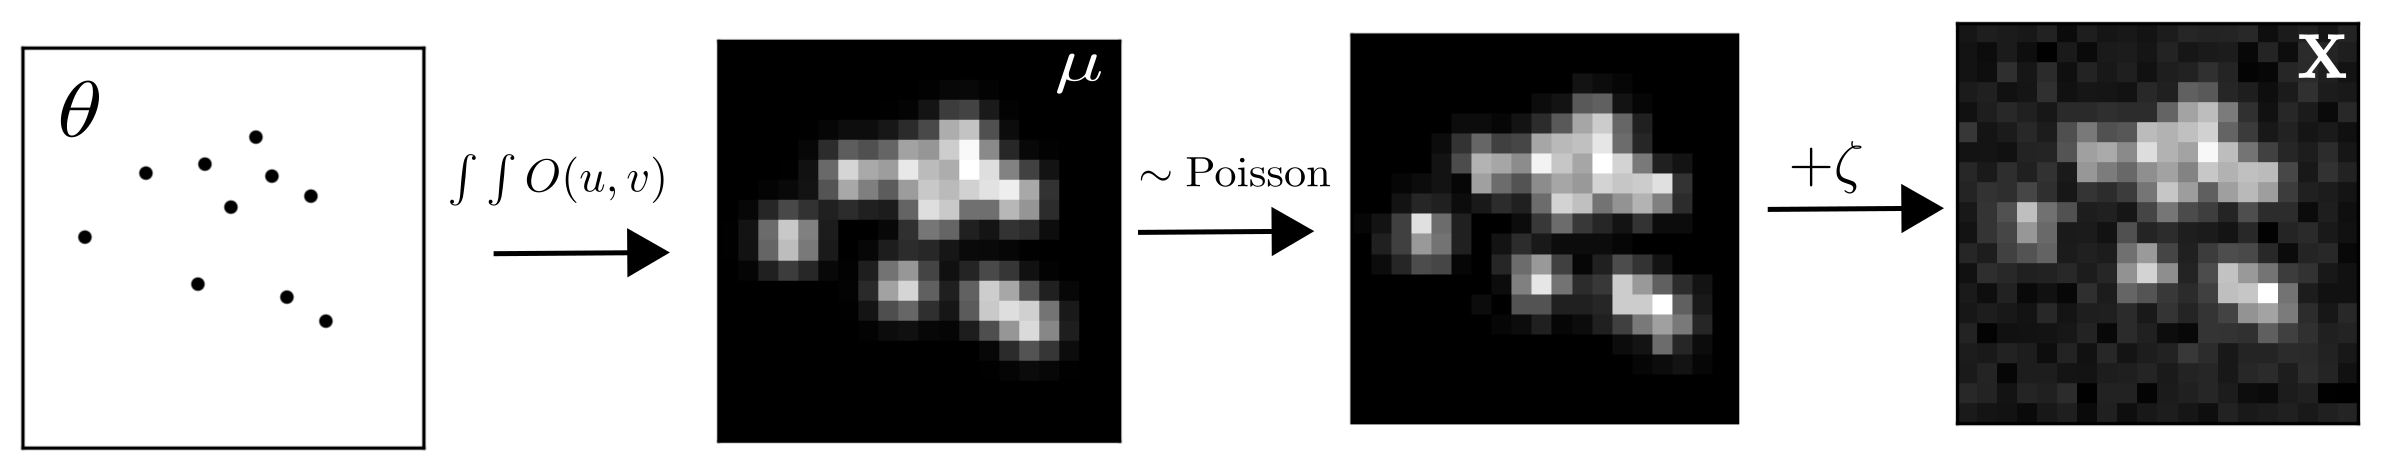
\includegraphics[scale=0.65]{Generation-Figure.png}
\caption{Generative model of single molecule localization microscopy images}
\end{figure}

The distribution of $\bold{x}$ is the convolution of the distributions of $\bold{s}$ and $\zeta$,

\begin{equation}
p(\bold{x}_{k}|\theta) = A\sum_{q=0}^{\infty} \frac{1}{q!}e^{-\omega_{k}}\omega_{k}^{q}\frac{1}{\sqrt{2\pi}\sigma_{k}}e^{-\frac{(\bold{x}_{k}-g_{k}q-o_{k})}{2\sigma_{k}^{2}}}
\end{equation}

where $p(\zeta_{k}) = \mathcal{N}(o_{k},\sigma_{k}^{2})$ and $p(s_{k}) = \mathrm{Poisson}(\omega_{k})$,  $A$ is some normalization constant. In practice, (4) is difficult to work with, so we look for an approximation. We will use a Poisson-Normal approximation for simplification. Consider,

\begin{equation}
\zeta_{k} - o_{k} + \sigma_{k}^{2} \sim \mathcal{N}(\sigma_{k}^{2},\sigma_{k}^{2}) \approx \mathrm{Poisson}(\sigma_{k}^{2})
\end{equation}

Since $\bold{x}_{k} = \bold{s}_{k} + \zeta_{k}$, we transform $\bold{x}_{k}' = \bold{x}_{k} - o_{k} + \sigma_{k}^{2}$, which is distributed according to 

\begin{equation}
\bold{x}_{k}' \sim \mathrm{Poisson}(\omega_{k}')
\end{equation}

where $\omega_{k}' = \omega_{k} + \sigma_{k}^{2}$. This result can be seen from the fact the the convolution of two Poisson distributions is also Poisson. We then arrive at the following log likelihood

\begin{equation}
\ell(\bold{x}|\theta) = -\log \prod_{k} \frac{e^{-\left(\mu_{k}'\right)}\left(\mu_{k}'\right)^{n_{k}}}{n_{k}!}
\approx \sum_{k}  n_{k}\log n_{k} + \mu_{k}' - n_{k}\log\left(\mu_{k}'\right)
\end{equation}

\subsection{Localization Error}

We use the Fisher information as an information theoretic criteria to assess the quality of the proposed algorithms, with respect to the root mean squared error (RMSE) of our predictions of $\theta$. The generative model $\ell(\bold{x}|\theta)$ is also convenient for computing the Fisher information matrix (Smith 2010) and thus the Cramer-Rao lower bound, which bounds the variance of a statistical estimator of $\theta$, from below i.e., $\mathrm{var}(\hat{\theta}) \geq I^{-1}(\theta)$. It is shown in the appendix, that the Fisher information is straightforward to compute under the Poisson likelihood (7)

\begin{equation}
\mathcal{I}_{ij}(\theta) = \underset{\theta}{\mathbb{E}}\left(\frac{\partial \ell}{\partial\theta_{i}}\frac{\partial\ell}{\partial\theta_{j}}\right) = \sum_{k}\frac{1}{\omega_{k}'}\frac{\partial \omega_{k}'}{\partial\theta_{i}}\frac{\partial \omega_{k}'}{\partial\theta_{j}}
\end{equation}

\subsection{Kernel density estimation with deep networks}

Direct optimization of the log-likelihood in (7) from observations $\bold{x}$ alone is challenging when fluorescent emitters are dense within the field of view and fluorescent signals significantly overlap. Convolutional neural networks (CNN) have recently been used in fluorescence microscopy to extract parameters describing fluorescent emitters such as color, emitter orientation, z coordinate, background signal. For localization tasks, CNNs typically employ upsampling layers to reconstruct Bernoulli probabilities of emitter occupancy or kernel density estimates with higher resolution than experimental measurements. Kernel density estimates are the most common data structure used in SMLM, and can be easlily generated from molecular coordinates using the optical impulse response (2). While ground-truth data from experiments to train the neural network are typically not available, synthetic training data can also be generated by (2) and simulation from the Poisson likelihood (7). 

The DeepSTORM CNN, initially proposed in [1] for 3D localization, can be viewed as a deep kernel density estimator, reconstructing kernel density estimates $\bold{y}$ from low-resolution inputs $\bold{x}$. We utilize a simplified form of the original architecture for 2D localization, which we denote $\phi$ hereafter, which consists of three main modules: a multi-scale context aggregation module, an upsampling module, and a prediction module. For context aggregation, the architecture utilizes dilated convolutions to increase the receptive field of each layer. The upsampling module is then composed of two consecutive 2x resize-convolutions, computed by nearest-neighbor interpolation, to increase the lateral resolution by a factor of 4. For a common sCMOS camera, each pixel has a lateral size of approximately 108 nanometers, giving approximately 27 nanometer pixels in the KDE. The terminal prediction module contains three additional convolutional blocks for refinement of the upsampled image, followed by an element-wise HardTanh. 


\section{Denoising Diffusion Probabilistic Model for SMLM}

We consider datasets $(\bold{x}_i,\bold{y}_i,\hat{\bold{y}}_{i})_{i=1}^{N}$ of observed images $\bold{x}_i$ true kernel density estimate (KDE) images $\bold{y}_{i}$, and KDE estimates $\hat{\bold{y}}_{i}=\phi(\bold{x}_{i})$. Observations $\bold{x}_i$ are generated under the image degradation model. We aim to develop a framework for sampling from $p(\hat{\bold{y}}|\bold{x},\bold{y})$.

\section{Conditional Denoising Diffusion Model}

Point estimates $\hat{\bold{y}}_{i}$ produced by the DeepSTORM architecture lack uncertainty quantification.  To address this, we propose a DDPM to model the conditional distribution $p(\hat{\bold{y}}|\bold{x},\bold{y})$. Consider the factorization $p(\hat{\bold{y}}|\bold{x},\bold{y})p(\bold{x}|\bold{y})p(\bold{y})=p(\bold{x}|\bold{y},\hat{\bold{y}})p(\bold{y}|\hat{\bold{y}})p(\hat{\bold{y}})$. Given that $\bold{x}$ is conditionally independent of $\hat{\bold{y}}$, we find

\begin{equation*}
p_{\Psi}(\hat{\bold{y}}|\bold{x},\bold{y})=p(\bold{y}|\hat{\bold{y}})
\end{equation*}

Evidently, the DDPM $\Psi$ can be trained on pairs $(\bold{y}_i,\hat{\bold{y}}_{i})_{i=1}^{N}$. The conditional DDPM generates a target KDE $\bold{y}_0$ in $T$ refinement steps. Starting with a pure noise image $\bold{y}_{T}\sim \mathcal{N}(0,\bold{I})$, the model iteratively refines the KDE through successive iterations according to learned conditional transition distributions $p(\bold{y}_{t-1}|\bold{y}_{t},\bold{})$ such that $\bold{y}_{0} \sim p(\bold{y}|\hat{\bold{y}})$ 

\subsection{Gaussian Diffusion}

\begin{figure}
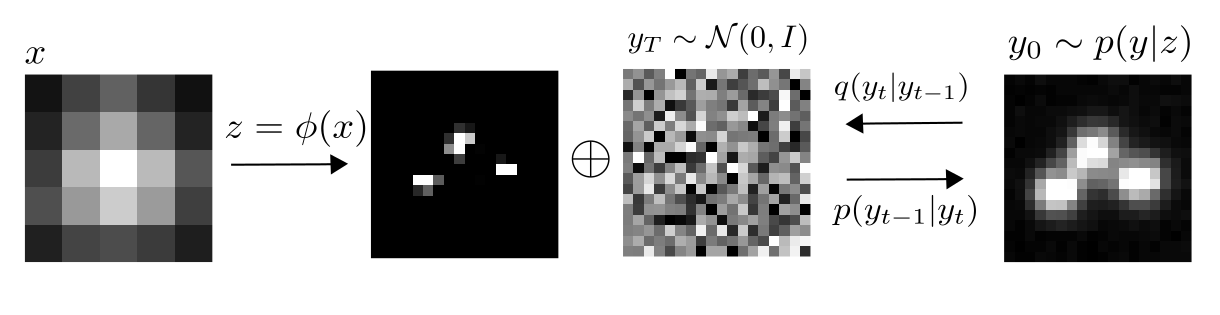
\includegraphics[scale=4.5]{Denoise.png}
\caption{Conditional diffusion model for sampling kernel density estimates}
\end{figure}

Diffusion models (Sohl-Dickstein 2015; Ho 2020) are a class of generative models inspired by nonequilibrium statistical physics, which slowly destroy structure in a data distribution $p(\bold{y}_{0}|\bold{x})$ via a fixed Markov chain referred to as the \emph{forward process}. In the present context, the forward process gradually adds Gaussian noise to the KDE $\bold{y}$ according to a variance schedule $\beta_{0:T}$

\begin{equation}
q(\bold{y}_{t}|\bold{y}_{0}) = \prod_{t=1}^{T}q(\bold{y}_{t}|\bold{y}_{t-1}) \;\;\; q(\bold{y}_{t}|\bold{y}_{t-1}) = \mathcal{N}\left(\sqrt{1-\beta_{t}}\bold{y}_{t-1},\beta_t I\right)
\end{equation}

An important property of the forward process is that it admits sampling $\bold{y}_t$ at an arbitrary timestep $t$ in closed form (Ho 2020). Using the notation $\alpha_t := 1 - \beta_t$ and $\gamma_t := \prod_{s=1}^{t} \alpha_s$, we have

\begin{equation}
q(\bold{y}_t|\bold{y}_0) = \mathcal{N} \left(\sqrt{\gamma_{t}} \bold{y}_{0}, (1 - \gamma_t)I \right)
\end{equation}


The usual procedure is then to learn a parametric representation of the \emph{reverse process}, and therefore generate samples from  $p(\bold{y}_{0})$, starting from noise. Formally, $p_{\theta}(\bold{y}_{0}|\bold{\hat{y}}) = \int p_{\theta}(\bold{y}_{0:T}|\bold{\hat{y}})d\bold{\hat{y}}_{1:T}$ where $\bold{y}_{t}$ is a latent representation with the same dimensionality of the data.  $p_{\theta}(\bold{y}_{0:T}|\bold{\hat{y}})$ is a Markov process, starting from a noise sample $p_{\theta}(\bold{y}_{T}) = \mathcal{N}(0,\bold{I})$. 

\begin{equation}
p_{\theta}(\bold{y}_{0:T}) = p_{\theta}(\bold{y}_{T})\prod_{t=1}^{T} p_{\theta}(\bold{y}_{t-1}|\bold{y}_{t}) \;\;\; p_{\theta}(\bold{y}_{t-1}|\bold{y}_{t}) = \mathcal{N}\left(\mu_{\theta}(\bold{y}_{t}),\beta_{t}I\right)
\end{equation}

where we reuse the variance schedule of the forward process (Ho 2020). We seek to learn a denoising model $\mu_{\theta}$ which computes the mean of the Gaussian transition density at each time step $t$. For all $t > 0$, the mean of the transition density is computed as

\begin{equation}
\mu_{\theta}(\bold{y}_t, \bold{\hat{y}}, \gamma_t) = \frac{1}{\sqrt{\alpha_t}} \left(\bold{y}_t - \frac{(1 - \alpha_t)}{\sqrt{1 - \gamma_t}} \, f_{\theta}(\bold{y}, \bold{\hat{y}}, \gamma_t) \right)
\end{equation}

where $f_{\theta}$ is a neural network. Only at $t=0$ is this mean directly a function of $\bold{x}$. 

\subsection{Optimization of the Denoising Model}

To reverse the diffusion process, we optimize a neural denoising model $f_{\theta}$ that takes as input $\bold{\hat{y}}$ and a noisy target image $\bold{y}_t \sim q(\bold{y}_t|\bold{y}_0)$. That is, this noisy target image $\bold{y}_t$ is drawn from the marginal distribution of noisy images at a time step $t$ of the forward diffusion process. 

\begin{equation}
\bold{y}_t = \sqrt{\gamma} \bold{y}_0 + \sqrt{1 - \gamma} \bold{\epsilon}, \quad \bold{\epsilon} \sim \mathcal{N}(0, \bold{I})
\end{equation}

In addition to a source image $\bold{y}_{0}$ and a noisy target image $\bold{y}_t$, the denoising model $f_{\theta}$ takes as input the sufficient statistics for the variance of the noise $\gamma$, and is trained to predict the noise vector $\bold{\epsilon}$. We make the denoising model aware of the level of noise through conditioning on a scalar $\gamma$. The proposed objective function for training $f_{\theta}$ is

\begin{equation}
\underset{(\bold{\hat{y}},\bold{y}_{0})}{\mathbb{E}}\underset{(\epsilon,\gamma)}{\mathbb{E}} \left[ f_{\theta}\left(x, \sqrt{\gamma} \bold{y}_0 + \sqrt{1 - \gamma} \epsilon \, \middle|\, \bold{y}_{t}, \gamma\right) - \epsilon \right],
\end{equation} 

where $(\bold{\hat{y}},\bold{y}_{0})$ is sampled from the training dataset and $\gamma \sim p(\gamma)$. The distribution of $\gamma$ has a big impact on the quality of the model and the generated outputs. For our training noise schedule, we use a piecewise distribution for $\gamma$, $p(\gamma) = \frac{1}{T}\sum_{t=1}^{T} U(\gamma_{t-1}, \gamma_t)$ (Nanxin 2021). Specifically, during training, we first uniformly sample a time step $t \sim \{0, ..., T\}$ followed by sampling $\gamma \sim U(\gamma_{t-1}, \gamma_t)$. We set $T = 100$ in all our experiments.

\subsection{Optimization of the DeepSTORM architecture}

A first pass at localization treats localization as a binary classification problem, such that 0 denotes a vacant pixel and 1 denotes an occupied pixel containing an emitter. Direct learning of pixel-wise classification with cross-entropy loss leads to an imbalance of occupied and unoccupied pixels in dense localization problems (Nehme 2020). CE loss is usually either weighted [51], replaced with a Focal loss [52], or applied to a "blobbed" version of the desired boolean volume e.g. by placing a disk around each GT position [53–55]. Alternative methods take a soft version of the binary classification problem. That is, by placing a small Gaussian around each GT position (e.g. with std of 1 pixel), and matching continuous heatmaps, backpropagation yields more meaningful gradients and eases the learning process convergence. 

Localization heatmaps thus form a natural encoding for SMLM images, which can be input to our conditional diffusion model. Therefore, to encode raw data $\bold{x}$ into a more tractable representation, we train the DeepSTORM architecture (Nehme 2020). Raw coordinates $\theta$ are binned into an upsampled image $\bold{z}$. 

\begin{equation*}
\mathcal{L}(\bold{y},\hat{\bold{y}}) = \lvert\lvert\bold{y}- \hat{\bold{y}}\lvert\lvert^2
\end{equation*} 


\section{Experiments}

\begin{figure}
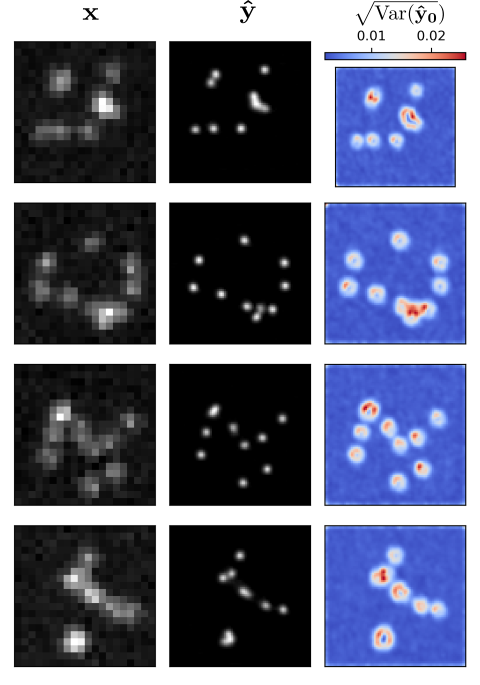
\includegraphics[scale=0.75]{Samples.png}
\caption{Kernel density estimates for various signal to noise ratios (SNR)}
\end{figure}

Training data was simulated under the image degradation model, drawing coordinates uniformly over a disc. We set $T = 100$ for all experiments and treat forward process variances $\beta_{t}$ as hyperparameters, with a linear schedule from $\beta_{0}=10^{-4}$ to $\beta_{T}=10^{-2}$.
These constants were chosen to be small relative to data scaled to $[-1, 1]$, ensuring that reverse and forward processes have approximately the same functional form while keeping the signal-to-noise ratio at $x_T$ as small as possible ($L_T = D_{KL}(q(x_T | x_0) \| \mathcal{N}(0, I)) \approx 10^{-5}$ bits per dimension in our experiments).

To represent the reverse process, we used the DDPM architecture based on a U-Net backbone (Ho 2020). Parameters are shared across time, which is specified to the network using the Transformer sinusoidal position embedding \cite{cite60}. We use self-attention at the $16 \times 16$ feature map resolution \cite{cite63,cite60}. Details are in Appendix A.

and the channel multipliers at different resolutions (see Appendix A for details). To condition the model on the input $x$, we up-sample the low-resolution image to the target resolution using bicubic interpolation. The result is concatenated with $y_t$ along the channel dimension. We experimented with more sophisticated methods of conditioning, such as using, but we found that the simple concatenation yielded similar generation quality.


\section{Related Work}

\subsection{Diffusion Models}

Prior work of diffusion models \cite{ref17, ref51} require 1-2k diffusion steps during inference, making generation slow for large target resolution tasks. We adapt techniques from \cite{ref6} to enable more efficient inference. Our model conditions on $\gamma$ directly (vs $t$ as in \cite{ref17}), which allows us flexibility in choosing the number of diffusion steps, and the noise schedule during inference. This has been demonstrated to work well for speech synthesis \cite{ref6}, but has not been explored for images. For efficient inference, we set the maximum inference budget to 100 diffusion steps, and hyper-parameter search over the inference noise schedule. This search is inexpensive as we only need to train the model once \cite{ref6}. We use FID on held-out data to choose the best noise schedule, as we found PSNR did not correlate well with image quality.

\section{Conclusion}

\section*{References}


{
\small


[1] Nehme, E., et al. {\it DeepSTORM3D: dense 3D localization microscopy and PSF design by deep learning}. Nature Methods 17, 734–740 (2020).


[2] Ouyang, W., et al. {\it Deep learning massively accelerates super-resolution localization microscopy}. Nature Biotechnology 36, 460–468 (2018).


[3] Speiser, A., et al. {\it Deep learning enables fast and dense single-molecule localization with high accuracy}. Nature Methods 18, 1082–1090 (2021).

[4] Sohl-Dickstein J., et al. {\it Deep unsupervised learning using nonequilibrium thermodynamics}. ICLR (2015).

[5] Ho J., et al. {\it Denoising Diffusion Probabilistic Models}. Advances in Neural Information Processing Systems (2015).

[6] Nanxin C., et al. {\it WaveGrad: Estimating Gradients for Waveform Generation
}. ICLR (2021).

[4] Chao, J., et al. {\it Fisher information theory for parameter estimation in single molecule microscopy: tutorial}. Journal of the Optical Society of America A 33, B36 (2016). 

[5] Schermelleh, L. et al. {\it Super-resolution microscopy demystified}. Nature Cell Biology vol. 21 72–84 (2019). 

[6] Zhang, B., et al. {\it Gaussian approximations of fluorescence microscope point-spread function models}. (2007). 

[7] Smith, C.S.,  {\it Fast, single-molecule localization that achieves theoretically minimum uncertainty}. Nature Methods 7, 373–375 (2010). 

[8] Nieuwenhuizen, R., et al. {\it Measuring image resolution in optical nanoscopy}. Nature Methods 10. 557-562 (2013). 

[9] Huang, F., et al. {\it Video-rate nanoscopy using sCMOS camera-specific single-molecule localization algorithms}. Nat Methods 10, 653–658 (2013). 

[10] Rust, M., et al. {\it Sub-diffraction-limit imaging by stochastic optical reconstruction microscopy (STORM)}. Nat Methods 3, 793–796 (2006).

[11] Betzig, E., et al. {\it Imaging intracellular fluorescent proteins at nanometer resolution. Science} 313, 1642–1645 (2006).

[12] Weigert, M., et al. {\it Content-aware image restoration: pushing the limits of fluorescence microscopy}. Nat. Methods 15, 1090 (2018).

[13] Falk, T., et al. {\it U-net: deep learning for cell counting, detection, and morphometry}. Nat. Methods 16, 67–70 (2019).

[14] Boyd, N., et al. {\it DeepLoco: fast 3D localization microscopy using neural networks}. Preprint at bioRxiv https://doi.org/10.1101/267096 (2018)

[15] Zelger, P., et al. {\it Three-dimensional localization microscopy using deep learning}. Opt. Express 26, 33166–33179 (2018)

[16] Zhang, P., et al. {\it Analyzing complex single-molecule emission patterns with deep learning}. Nat. methods 15, 913 (2018)

[17] Saharia, C., et al. {\it Image Super-Resolution via Iterative Refinement}. Preprint at arXiv https://doi.org/10.48550/arXiv.2104.07636 (2021)

}

\end{document}